\documentclass{ctexart}
\usepackage{geometry}
\usepackage{array}
\usepackage{makecell}
\usepackage{enumitem}
\usepackage{booktabs}
\usepackage{ragged2e}
\usepackage{tabularx}
\usepackage{fancyhdr} % 用于自定义页眉页脚
\usepackage{graphicx} % 应该已存在 (如果之前添加过)
\usepackage[HTML]{xcolor} % 新增:用于颜色定义和 colorbox
\usepackage{emptypage} % 如果之前添加了用于移除末尾空白页,请保留

% 页面边距设置
\geometry{a4paper, margin=1in}

% 自定义表格列类型
\newcolumntype{L}[1]{>{\RaggedRight\arraybackslash}p{#1}} % 左对齐,自动换行
\newcolumntype{M}[1]{>{\centering\arraybackslash}m{#1}}  % 水平居中,垂直居中,自动换行 (用户定义)

% fancyhdr 设置
\pagestyle{fancy} % 应用 fancy 页面样式
\fancyhf{} % 清空所有页眉页脚设置
\fancyhead[L]{\nouppercase{\leftmark}} % 页眉左侧显示当前节标题
\fancyfoot[C]{\thepage} % 页脚中间显示页码
\renewcommand{\headrulewidth}{0.4pt} % 页眉下方加一条线
\renewcommand{\footrulewidth}{0pt}  % 页脚上方不加线

% 为朴素页面样式(如目录页)重新定义
\fancypagestyle{plain}{%
  \fancyhf{}%
  \fancyfoot[C]{\thepage}%
  \renewcommand{\headrulewidth}{0pt}%
  \renewcommand{\footrulewidth}{0pt}%
}

% 定义横幅颜色
\definecolor{MyBannerTeal}{HTML}{FF8880}

\begin{document}

\begin{titlepage}
    \thispagestyle{empty} % 标题页不显示页眉页脚
    \vspace*{-1.15in} % 新增:向上移动1英寸以抵消顶部边距
    % 顶部图片: 设置为铺满整个纸张宽度
    \noindent\hspace*{-1in}%
    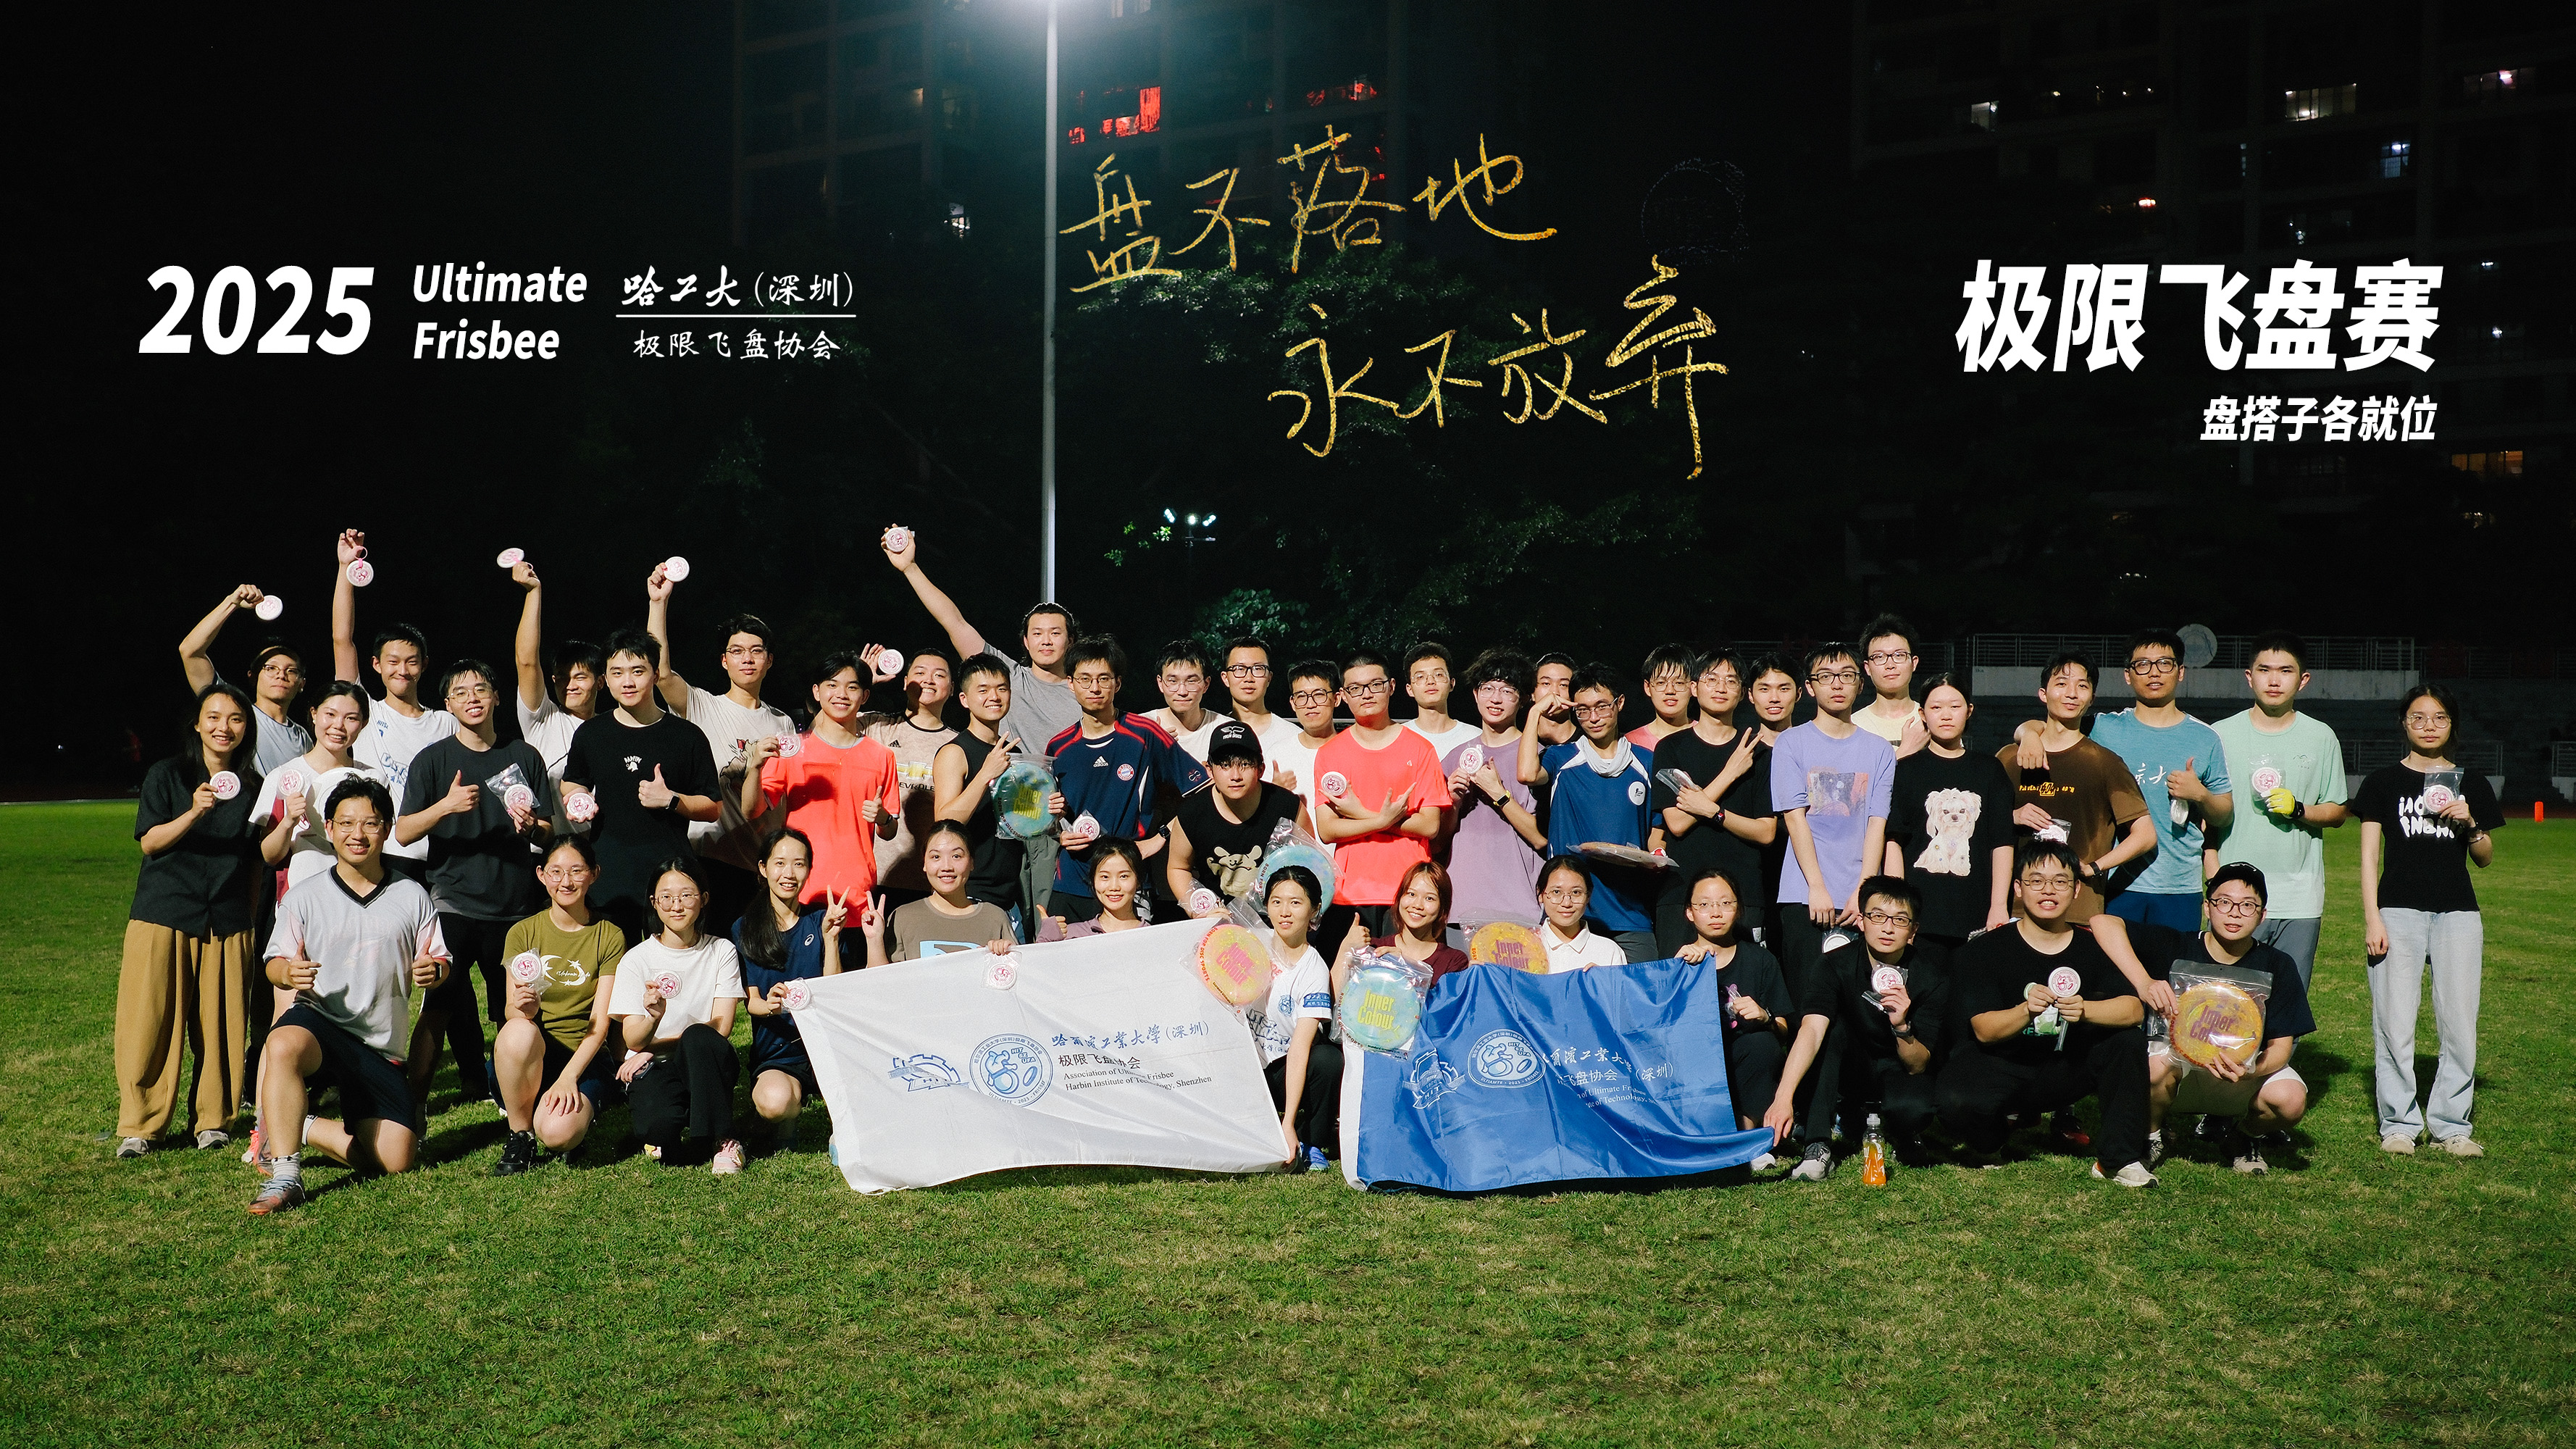
\includegraphics[width=\paperwidth, height=0.4\paperheight, keepaspectratio]{大合照.jpg}%

    % 彩色条带 (无文字,宽度为 paperwidth)
    \vspace{-1pt} % 此行用于消除图片和彩带间的微小间距,应保留
    \noindent\hspace*{-1in}%
    \colorbox{MyBannerTeal}{% % 使用您最终确定的颜色名称
        \begin{minipage}[c][2em][c]{\dimexpr\paperwidth-2\fboxsep\relax} % 彩色条带高度,例如3em,宽度为paperwidth
            \hspace{0pt} % 确保minipage有内容以正确计算高度
        \end{minipage}%
    }

    % 彩色条带下方的文本信息
    \begin{center}
        \vspace{4em} % 彩色条带与主标题之间的间距
        {\LARGE 哈尔滨工业大学(深圳)2025极限飞盘新生杯\par} % 主标题移到此处
        
        \vspace{1.5em} % 主标题与副标题之间的间距
        {\Large 赛程安排与注意事项 (10月21日, 10月28日, 11月4日, 11月11日)} \\[2em] % 副标题
        
        {哈尔滨工业大学(深圳)极限飞盘协会} \\[1em]
        {2025年10月18日}\par

        \vspace{12em} % 在日期和旗帜之间添加一些垂直间距
        % 插入修剪后的协会旗帜 PDF
        
\includegraphics[width=0.65\paperwidth, trim=50bp 6.4cm 50bp 6.3cm, clip]{协会旗帜.pdf}
    \end{center}

    \vfill
\end{titlepage}

\clearpage
\pagenumbering{roman}
\pagestyle{plain}
% \tableofcontents
\clearpage
\pagenumbering{arabic}
\pagestyle{fancy}

\section{赛事简介、赛制与场地说明}
本次极限飞盘新生杯采用4队小组循环赛加决赛轮的赛制,旨在为新生提供充分的学习交流和竞技机会。
\begin{itemize}
    \item \textbf{参赛队伍:} A队, B队, C队, D队。
    \item \textbf{小组循环赛:} 所有队伍两两之间进行一场比赛,共6轮比赛,每队参与3场。
    \item \textbf{比赛用时与规则:}每场比赛时长50分钟,5人制。
    \item \textbf{比赛信号:} 比赛开始与结束时,将以汽笛鸣一声为信号。
    \item \textbf{排位规则:} 小组循环赛结束后,根据各队积分进行排名。小组赛积分规则为:胜一场积2分,平一场积1分,负一场积0分。若积分相同,则依次比较:1) 相互间胜负关系(仅当两队同分时适用);2) 总净胜分;3) 总得分数。
    \item \textbf{队伍颜色:} 为确保比赛中队伍区分清晰,每场比赛将为对阵双方指定深/浅色队服。请所有参赛队员务必\textbf{准备好深色(建议为黑色或深蓝色)和浅色(建议为白色)运动上衣各一件}。
    \item \textbf{比赛地点与场地安排:}
    \begin{itemize}
        \item \textbf{比赛地点:} 哈工大操场。
        \item \textbf{场地设置:} 使用操场上的两个场地同时进行比赛。
        \begin{itemize}
            \item \textbf{场地1:} 位于靠近维也纳酒店一侧。
            \item \textbf{场地2:} 位于远离维也纳酒店一侧。
        \end{itemize}
        \item \textbf{场地指引:} 请各队伍根据赛程表提前到达指定场地进行热身和赛前准备。
    \end{itemize}
\end{itemize}

\section{第一活动日:2025年10月21日(周二)- 教学与规则讲解}

\subsection*{活动安排 (10月21日)}
\renewcommand{\arraystretch}{1.8}
\begin{tabularx}{\textwidth}{@{} L{2.2cm} L{1.5cm} X L{3.2cm} @{}}
    \toprule
    \textbf{时间段} & \textbf{场地} & \textbf{活动内容} & \textbf{备注} \\
    \midrule
    18:45 - 20:45 & 场地1 & 教学与规则讲解 & 基础技能训练 \\
    18:45 - 20:45 & 场地2 & 教学与规则讲解 & 基础技能训练 \\
    \bottomrule
\end{tabularx}
\renewcommand{\arraystretch}{1.0}

\subsection*{当日重要提醒 (10月21日)}
\begin{itemize}
    \item 请所有队员于 18:30 前到达场地签到。
    \item 今日主要进行飞盘基础技能教学和规则讲解,无正式比赛。
\end{itemize}

\newpage

\section{第二活动日:2025年10月28日(周二)- 小组循环赛 (第1-4场)}

\subsection*{赛程安排 (10月28日)}
\renewcommand{\arraystretch}{1.8}
\begin{tabularx}{\textwidth}{@{} L{2.2cm} L{1.5cm} X L{3.2cm} @{}}
    \toprule
    \textbf{时间段} & \textbf{场地} & \textbf{对阵双方 (左队深色, 右队浅色)} & \textbf{阶段 / 备注} \\
    \midrule
    \multicolumn{4}{l}{\textit{18:30 到达、集合、队长报到、热身准备}} \\
    \addlinespace
    \multicolumn{4}{c}{\textbf{第一轮小组赛}} \\
    18:45 - 19:35 & 场地1 & A队 (深) vs B队 (浅) & 小组赛第1场 (50分钟) \\
    18:45 - 19:35 & 场地2 & C队 (深) vs D队 (浅) & 小组赛第2场 (50分钟) \\
    \addlinespace
    \multicolumn{4}{l}{\textit{19:35 - 19:55 中场休息、拍照、换场准备}} \\
    \addlinespace
    \multicolumn{4}{c}{\textbf{第二轮小组赛}} \\
    19:55 - 20:45 & 场地1 & A队 (深) vs D队 (浅) & 小组赛第3场 (50分钟) \\
    19:55 - 20:45 & 场地2 & C队 (深) vs B队 (浅) & 小组赛第4场 (50分钟) \\
    \addlinespace
    \multicolumn{4}{l}{\textit{20:45后 Circle交流、合影留念}} \\
    \addlinespace
    \bottomrule
\end{tabularx}
\renewcommand{\arraystretch}{1.0}

\subsection*{当日重要提醒 (10月28日)}
\begin{itemize}
    \item 请所有队伍于 18:30 前到达场地签到、热身,到场第一件事先签风险告知书,每队一份!
    \item \textbf{重要服装提示:} 本日比赛颜色分配请严格参照上表,左队深色,右队浅色。
\end{itemize}

\newpage

\section{第三活动日:2025年11月4日(周二)- 小组循环赛 (第5-6场) 与半决赛}

\subsection*{赛程安排 (11月4日)}
\renewcommand{\arraystretch}{1.8}
\begin{tabularx}{\textwidth}{@{} L{2.2cm} L{1.5cm} X L{3.2cm} @{}}
    \toprule
    \textbf{时间段} & \textbf{场地} & \textbf{对阵双方 (左队深色, 右队浅色)} & \textbf{阶段 / 备注} \\
    \midrule
    \multicolumn{4}{l}{\textit{18:30 到达、集合、队长报到、热身准备}} \\
    \addlinespace
    \multicolumn{4}{c}{\textbf{第三轮小组赛}} \\
    18:45 - 19:35 & 场地1 & A队 (深) vs C队 (浅) & 小组赛第5场 (50分钟) \\
    18:45 - 19:35 & 场地2 & B队 (深) vs D队 (浅) & 小组赛第6场 (50分钟) \\
    \addlinespace
    \multicolumn{4}{l}{\textit{19:35 - 19:55 中场休息、拍照、计算排名}} \\
    \addlinespace
    \multicolumn{4}{c}{\textbf{半决赛轮}} \\
    19:55 - 20:45 & 场地1 & 积分第1名 vs 积分第4名 & 半决赛第7场 (50分钟) \\
    19:55 - 20:45 & 场地2 & 积分第2名 vs 积分第3名 & 半决赛第8场 (50分钟) \\
    \addlinespace
    \multicolumn{4}{l}{\textit{20:45后 Circle交流、决赛对阵确定}} \\
    \addlinespace
    \bottomrule
\end{tabularx}
\renewcommand{\arraystretch}{1.0}

\subsection*{当日重要提醒 (11月4日)}
\begin{itemize}
    \item 请所有队伍于 18:30 前到达场地签到、热身。
    \item \textbf{重要服装提示:}请各位同学今天务必带好深色和浅色两件运动上衣,中场会留出充足时间给大家更换。
\end{itemize}

\newpage

\section{第四活动日:2025年11月11日(周二)- 决赛轮与颁奖}

\subsection*{赛程安排 (11月11日)}
\renewcommand{\arraystretch}{1.8}
\begin{tabularx}{\textwidth}{@{} L{2.2cm} L{1.5cm} X L{3.2cm} @{}}
    \toprule
    \textbf{时间段} & \textbf{场地} & \textbf{对阵双方 (左队深色, 右队浅色)} & \textbf{阶段 / 备注} \\
    \midrule
    \multicolumn{4}{l}{\textit{18:30 到达、集合、队长报到、决赛准备}} \\
    \addlinespace
    \multicolumn{4}{c}{\textbf{决赛轮}} \\
    18:45 - 19:45 & 场地1 & 第7场负者 vs 第8场负者 & \textbf{三四名决赛} (60分钟) \\
    18:45 - 19:45 & 场地2 & 第7场胜者 vs 第8场胜者 & \textbf{冠军决赛} (60分钟) \\
    \addlinespace
    \multicolumn{4}{l}{\textit{19:45后 Circle交流、选取MVP、颁奖、大合影}} \\
    \addlinespace
    \bottomrule
\end{tabularx}
\renewcommand{\arraystretch}{1.0}

\subsection*{当日重要提醒 (11月11日)}
\begin{itemize}
    \item 请所有队伍于 18:30 前到达场地签到、热身。
    \item 决赛轮将决定最终的冠、亚、季、殿军。
    \item 比赛结束后将进行颁奖仪式和大合影。
\end{itemize}

\newpage

\section{赛事总体注意事项}
\begin{enumerate}[label=\arabic*., itemsep=0.5em]
    \item \textbf{参赛服装:} 请所有参赛队员务必\textbf{准备深色和浅色运动上衣各一件}。每场比赛的具体颜色分配请严格参照赛程表。
    \item \textbf{饮水:} 场地不提供一次性水杯,请各位选手\textbf{务必自带充足饮用水及水壶}。
    \item \textbf{安全第一:} 请大家在比赛中务必注意自身和他人的安全,热身充分,量力而行,避免受伤。
    \item \textbf{保险:} 请所有运动员务必提前购买运动保险。
    \item \textbf{准时与场地:} 请各队严格遵守比赛时间,提前到场准备。
    \item \textbf{体育精神:} 秉持"Spirit Of The Game (SOTG)"飞盘精神,尊重比赛,尊重对手,尊重队友,公平竞争。
    \item \textbf{场地保持:} 请爱护场地设施,比赛结束后自觉清理垃圾,保持场地整洁。
\end{enumerate}

\vspace{1.5em}
\begin{center}
期待各位的积极参与,预祝比赛顺利,大家玩得开心!
\end{center}

\noindent\rule{\linewidth}{0.4pt}
\vspace{1em}

\begin{flushleft}
\textbf{主办单位:} \\
哈尔滨工业大学(深圳)团委 \\[1em]

\textbf{承办单位:} \\
哈尔滨工业大学(深圳)极限飞盘协会
\end{flushleft}

\appendix
\section{参赛人员名单}

\subsection*{A队}
\renewcommand{\arraystretch}{1.2}
\begin{tabularx}{\textwidth}{@{} L{3cm} M{2cm} X @{}}
    \toprule
    \textbf{姓名} & \textbf{性别} & \textbf{学号} \\
    \midrule
    刘慕实 & 男 & 25S151141 \\
    耿增越 & 男 & 2023311226 \\
    蔡洛萱 & 女 & 2024314677 \\
    赵浩帆 & 男 & 25B965005 \\
    刘睿泽 & 男 & 2024311062 \\
    寇家辉 & 男 & 2024311312 \\
    陈子博 & 男 & 25S165056 \\
    郝建晓 & 男 & 25S153158 \\
    庄冠宁 & 男 & 25S065015 \\
    蔡卓畅 & 男 & 25S165041 \\
    郭芯言 & 女 & 220210228 \\
    郭昱辰 & 女 & 2023311H03 \\
    郑雨竺 & 女 & 25S156021 \\
    \bottomrule
\end{tabularx}

\subsection*{B队}
\renewcommand{\arraystretch}{1.2}
\begin{tabularx}{\textwidth}{@{} L{3cm} M{2cm} X @{}}
    \toprule
    \textbf{姓名} & \textbf{性别} & \textbf{学号} \\
    \midrule
    王昭蔚 & 男 & 25s155019 \\
    贾思洋 & 男 & 23SM46556 \\
    丁俊洋 & 男 & 220310206 \\
    黄俊杰 & 男 & 2023313619 \\
    李慧城 & 男 & 2024312115 \\
    徐传奇 & 男 & 2024312906 \\
    吴锦霈 & 男 & 2025310749 \\
    黄乐佳 & 男 & 2025310486 \\
    朱海峰 & 男 & 25S051029 \\
    黄睿涵 & 女 & 2024312712 \\
    考沛瑶 & 女 & 24S039019 \\
    刘芷烨 & 女 & 25S152047 \\
    陈子瑶 & 女 & 2025310432 \\
    \bottomrule
\end{tabularx}

\subsection*{C队}
\renewcommand{\arraystretch}{1.2}
\begin{tabularx}{\textwidth}{@{} L{3cm} M{2cm} X @{}}
    \toprule
    \textbf{姓名} & \textbf{性别} & \textbf{学号} \\
    \midrule
    马荣 & 男 & 2025330524 \\
    黄家骏 & 男 & 2024311040 \\
    倪梓源 & 男 & 2023313729 \\
    Nadeem Masih & 男 & 23BF52005 \\
    刘尊 & 男 & 24S152072 \\
    陈豪 & 男 & 2025310364 \\
    黄舒涵 & 男 & 2025213672 \\
    张陈宇 & 男 & 2024311097 \\
    Zakaria Moustahib & 男 & 2025330183 \\
    潘秀丽 & 女 & 2024312180 \\
    孟欣 & 女 & 24B926002 \\
    田佳 & 女 & 25S057001 \\
    黎加馨 & 女 & 2025311584 \\
    \bottomrule
\end{tabularx}

\subsection*{D队}
\renewcommand{\arraystretch}{1.2}
\begin{tabularx}{\textwidth}{@{} L{3cm} M{2cm} X @{}}
    \toprule
    \textbf{姓名} & \textbf{性别} & \textbf{学号} \\
    \midrule
    张豫艳 & 女 & 25S153147 \\
    马悠然 & 男 & 2023311228 \\
    刘证涛 & 男 & 2024311417 \\
    朱昱玮 & 男 & 2023311E13 \\
    杨鸿鑫 & 男 & 2024312706 \\
    宁智煌 & 男 & 25S165027 \\
    张硕 & 男 & 25S155080 \\
    李旺 & 男 & 25s152079 \\
    郭辉源 & 男 & 25S151181 \\
    SARKER BIKAS & 男 & 2025330273 \\
    杨婧兰 & 女 & 2024311450 \\
    李焱 & 女 & 25S155079 \\
    李园 & 女 & 25S153034 \\
    \bottomrule
\end{tabularx}

\end{document}